%%%%%%%%%%%%%%%%%%%%%%%%%%%%%%%%%%%%%%%

\chapter{~~Expérimentations}


Dans la littérature, les instances font partie intégrante de la résolution des problèmes et c'est d'autant plus vrai en recherche opérationnelle. 
En effet les instances assurent les motivations de la recherche et permettent aussi de poser les bases afin de comparer les méthodes de résolution comme par exemple les instances de Solomon pour le problème de \vrptw \cite{solomon1987} qui sont devenues la référence lorsque l'on souhaite montrer ses résultats sur le problème de tournées de véhicules.

Dans un premier temps nous présenterons nos instances tirées de la vie réelle puis nous afficherons les résultats obtenus sur ces instances avec les différentes méthodes de résolution : celles que nous avons implémentées et celles déjà existantes.

%%%%%%%%%%%%%%%%%%%%%%%%%%%%%%%%%%%%%%%
%%%%%%%%%%%%%%%%%%%%%%%%%%%%%%%%%%%%%%%

%\section{Introduction \label{sec:R_intro}}
%\input{R_intro.tex}
%%%%%%%%%%%%%%%%%%%%%%%%%%%%%%%%%%%%%%%
%%%%%%%%%%%%%%%%%%%%%%%%%%%%%%%%%%%%%%%

\section{Instances \label{sec:R_instances}}
Les instances que nous utilisons pour tester nos méthodes de résolution sont réelles. Et donc les solutions que nous proposons sont mises en place. 
Nous avons donc eu accès à de nombreuses instances des deux sociétés clientes de DecisionBrain.
Les instances de la société britannique possèdent les contraintes spécifiques du problème alors que les instances de la société danoise sont plus contraintes en terme de compétences et de niveau de compétences.
De plus nous avons aussi créé des instances de petite taille.
La table~\ref{table:instances} présente les données de chaque instance.
Le format de chaque instance est le suivant : 
\begin{itemize}
\item Le nom de l'instance correspond au nombre de techniciens et au nombre de tâches (instance\#3\#15 correspond à l'instance avec trois techniciens et quinze tâches).
\item $|\prece|$ indique le nombre de contraintes de précédence.
\item $|\same|$ donne le nombre de contraintes de même technicien.
\item $|\app|$ représente le nombre de contraintes de pré-assignation.
\item $\nskill$ dénote le nombre de domaines de compétences.
\item $\#position$ désigne le nombre de positions pour les tâches et techniciens dans le graphe de distance (matrice de transition).
\item $\twTech{\tech}$ (resp. $\twTask{\task}$) renseigne le nombre moyen de fenêtres temporelles des techniciens (resp. tâches).

\end{itemize}


\begin{table}
[H]
\centering
\begin{tabular}
{|l|l|l|l|l|l|l|l|}
\hline
instance & $|\prece|$ & $ |\same|$ & $|\app|$ & $q$ & \#position & $\twTech{\tech}$ & $\twTask{\task}$\\
\hline
instance\#3\#15 & 0 & 0 & 0 & 2 & 4 & 1 & 1 \\
instance\#30\#256 & 0 & 0 & 0 & 154 & 162 & 0.96 & 1 \\
instance\#30\#305 & 30 & 5 & 0 & 137 & 162 & 0.9 & 1 \\
instance\#30\#2781 & 341 & 101 & 37 & 137 & 514 & 0.9 & 0.92 \\
instance\#144\#1377 & 0 & 0 & 0 & 154 & 163 & 0.875 & 1 \\
instance\#145\#4568 & 0 & 0 & 0 & 183 & 544 & 0.87 & 1 \\
\hline
\end{tabular}
\caption{Tableau présentant les instances.\label{table:instances}}

\end{table}


L'instance nommée "instance\#3\#15" est une instance que nous avons généré pour tester nos modèles dans un premier temps.
Les instances instance\#30\#305 et instance\#30\#2781 sont des instances de la société britannique.
Les instances instance\#144\#1377 et instance\#145\#4568 sont des instances de la société danoise.
Cependant ce sont des instances de tests.
Ce sont des instances générées à la main par le client à partir de données réelles, mais pas des instances générées automatiquement par leur système opérationnel.

Les contraintes de compétences et les positions des tâches et techniciens sont dimensionnantes dans notre problème.
Le nombre de positions montre l'espace de recherche des tournées pour chaque technicien.
Même si les contraintes de compétences filtrent les tâches qu'un technicien peut effectuer, le technicien doit tout de même décider quels chemins prendre dans un graphe complet de 160 à 550 sommets.







%%%%%%%%%%%%%%%%%%%%%%%%%%%%%%%%%%%%%%%
%%%%%%%%%%%%%%%%%%%%%%%%%%%%%%%%%%%%%%%

%\section{Résultats\label{sec:R_results}}


Dans la suite de cette section nous présentons les résultats obtenus avec les différentes méthodes de résolution.

Le premier modèle (programmation linéaire en nombres entiers) n'est peut-être pas intéressant du point de vue de ces performances numériques.
Cependant il nous permet d'obtenir une borne supérieure grâce à la relaxation linéaire du programme linéaire en nombres entiers.
Cette borne supérieure nous permet d'obtenir un gap à partir de toute solution réalisable obtenue par une autre méthode de résolution.
Le gap représente la distance maximale qu'il existe entre une solution réalisable et la borne supérieure (potentiellement la solution optimale).
Soit $sol_{RL}$ la valeur de la relaxation linéaire et $sol_{int}$ la valeur de la solution entière courante le gap est calculé comme suit :
$$
\text{gap} = \frac{|sol_{RL} - sol_{int}|}{|sol_{int}|}
$$

Par exemple, si on obtient un gap de 10\%, cela veut dire que la solution optimale est à moins de 10\% de la solution courante.

Nous avons implémenté un algorithme de génération de colonnes.
La génération de colonnes est une méthode de résolution indépendante des modèles utilisés par le RMP et le PSP.
Il faut fournir un modèle pour le RMP et le modèle du PSP associé à l'algorithme de génération de colonnes et celle-ci fonctionne.
C'est aussi le cas pour le branch and price car celui-ci utilise la génération de colonnes à chacun des n\oe uds de l'arbre.
Cette méthode de résolution pourra être utilisée par DecisionBrain pour d'autres problèmes.





\subsection{Résultats numériques}
Les méthodes de résolution utilisent soit CPLEX soit CP Optimizer.
Pour cela nous utilisons Cplex Studio 12.6.3.
Les tables~\ref{table:res_3_15}, \ref{table:res_30_256}, \ref{table:res_30_305} et \ref{table:res_grd_ins} présentent les résultats obtenus avec les méthodes de résolution.

Si la colonne "Status" indique "Optimal", alors la solution obtenue est optimale (avec la garantie d'optimalité) sinon elle indique "Réalisable".
Certaines solutions ont une valeur de fonction objectif optimale mais la garantie d'optimalité n'est pas vérifiée.
Le temps d'exécution est donné par la colonne "CPU(s)" (en seconde).
Ce temps ne prend pas en compte la génération du modèle.
La génération du modèle peut être assez longue selon le modèle choisi.
La colonne "Obj." désigne la valeur de la fonction objectif que l'on souhaite maximiser.
La colonne "Modèle" dénote le modèle utilisé pour la résolution.
Les modèles utilisés sont "PLNE" (programmation linéaire en nombres entiers), "PPC" (programmation par contraintes), "Heuristique" (une heuristique développée par DecisionBrain ; pour des raisons de confidentialité, nous ne pouvons la détailler) et "LNS" (recherche locale : large neighbourhood search en anglais).
Ensuite "Heuristique+PLNE" pour indiquer que nous utilisons une solution initiale calculée par l'heuristique qui fera office de point de départ du modèle en programmation linéaire en nombres entiers (resp. programmation par contraintes ou recherche locale).
Le "Gap" représente la distance maximale qui existe entre une solution réalisable et la borne supérieure (potentiellement la solution optimale).
Par exemple, si on obtient un gap de 10\% cela veut dire que la solution optimale est à moins de 10\% de la solution courante.

\begin{table}
[H]
\centering
 \begin{tabular}
 {|l|l|l|l|l|}
 \hline
 Instance & Modèle & Obj. & CPU(s) & Status \\
 \hline
instance\#3\#15 & PLNE & 12770.0 & 0 & Optimal\\
instance\#3\#15 & PPC & 12770.0 & 1 & Optimal\\
instance\#3\#15 & Heuristique & 11162.0 & 2 & Réalisable\\
instance\#3\#15 & Heuristique+PLNE & 12770.0 & 0 & Optimal\\
instance\#3\#15 & Heuristique+PPC & 12770.0 & 1 & Optimal\\
instance\#3\#15 & Heuristique+LNS & 12770.0 & 12 & Réalisable\\
 \hline
 \end{tabular}
 \caption{Résultats pour l'instance générée.\label{table:res_3_15}}
\end{table}

Nous présentons les résultats avec plusieurs limites de temps de résolution.
Nous utilisons comme limites de temps de résolution : 10 minutes, 30 minutes et 1 heure selon la taille des instances.
Pour les petites et moyennes instances, nous comparons les résultats avec 10 et 30 minutes de limite de temps de résolution et pour les grandes instances avec 1 heure de limite de temps de résolution.
La méthode de résolution actuellement utilisée par DecisionBrain est l'utilisation de l'heuristique pour obtenir une bonne première solution et ensuite la recherche locale pour améliorer cette solution.
Cette méthode de résolution correspond au modèle "Heuristique+LNS" dans les tableaux.
Nous comparons nos résultats par rapport à cette méthode de résolution.


\begin{table}
[H]
\centering
 \begin{tabular}
 {|l|l|l|l|l|l|}
 \hline
 Instance & Modèle & Obj. & CPU(s) & Status & Gap \\
 \hline
instance\#30\#256 & PLNE & 7733384.0 & 600.0 & Réalisable & 201\% \\
instance\#30\#256 & PPC &1.9903E7 & 605.0	& Réalisable & 18\%\\	
instance\#30\#256 & Heuristique & 2.1475E7 & 17.0 & Réalisable & 9.5\%\\
instance\#30\#256 & Heuristique+PLNE & 2.1475E7 & 600.0 & Réalisable & 9.5\% \\
instance\#30\#256 &	Heuristique+PPC & 2.1475E7 & 599.0 & Réalisable & 9.5\%\\
instance\#30\#256 & Heuristique+LNS & 2.1587E7 & 589.0 & Réalisable & 9\% \\
\hline
instance\#30\#305 & PLNE & 1152706.0 & 600.0 & Réalisable & 1100\% \\
instance\#30\#305 & PPC & 1.1227E7 & 600.0 & Réalisable & 36.5\%\\
instance\#30\#305 & Heuristique & 1.1269E7 & 21.0 & Réalisable & 35.6\%\\
instance\#30\#305 & Heuristique+PLNE & 1.1269E7 & 600.0 & Réalisable & 35.6\% \\
instance\#30\#305 & Heuristique+PPC & 1.2248E7 & 600.0 & Réalisable & 25.1\%\\
instance\#30\#305 & Heuristique+LNS & 1.3314E7 & 600.0 & Réalisable & 14.9\%\\
 \hline
 \end{tabular}
 \caption{Résultats pour les instances avec 30 techniciens et 256 tâches et 30 techniciens et 305 tâches avec un temps limite de résolution de 10 minutes.\label{table:res_30_256}}
\end{table}

Pour l'instance générée (de petite taille : 3 technicien et 15 tâches) nous observons que la solution optimale est obtenue par presque toutes les méthodes de résolution.
Cependant certaines méthodes (les heuristiques) ne donnent aucune garantie sur l'optimalité de la solution.

Pour les instances moyennes (30 technicien et environ 300 tâches), la modélisation en PLNE et peu performante : gap supérieur à 100\% alors que pour les autres méthodes de résolution le gap est proche de 10-20\%.
Même quand une solution initiale de bonne qualité est donnée les modélisation pour les méthodes exactes ont du mal à améliorer la solution pour l'instance instance\#30\#256.
Cependant grâce au PLNE nous obtenons une borne supérieure (relaxation linéaire) de : 2.3530E7 pour l'instance instance\#30\#256 et de : 1.5324E7 pour l'instance instance\#30\#305.
Ces bornes supérieures nous permettent de calculer le gap pour les autres méthodes de résolution.
 
 
 \begin{table}
[H]
\centering
 \begin{tabular}
 {|l|l|l|l|l|l|}
 \hline
  Instance & Modèle & Obj. & CPU(s) & Status & Gap \\
  \hline
instance\#30\#256 & PLNE & 1.1379E7 & 1802.0 & Réalisable & 105\% \\
instance\#30\#256 & PPC & 2.1393E7 & 1803.0 & Réalisable & 9.9\%\\
instance\#30\#256 & Heuristique & 2.1475E7 & 17.0 & Réalisable & 9.5\%\\
instance\#30\#256 & Heuristique+PLNE & 2.1475E7 & 1806.0 & Réalisable & 9.5\% \\
instance\#30\#256 & Heuristique+PPC & 2.1475E7 & 1803.0 & Réalisable & 9.5\%\\	
instance\#30\#256 & Heuristique+LNS & 2.1687E7 & 1643.0 & Réalisable & 8.5\%\\
 \hline
instance\#30\#305 & PLNE & 2364770.0 & 1801.0 & Réalisable & 525\% \\
instance\#30\#305 & PPC & 1.3094E7 & 1802.0 & Réalisable & 17\%\\
instance\#30\#305 & Heuristique & 1.1269E7 & 21.0 & Réalisable & 35\%\\
instance\#30\#305 & Heuristique+PLNE & 1.1278E7 & 1807.0 & Réalisable & 35\% \\
instance\#30\#305 & Heuristique+PPC & 1.3102E7 & 1802.0 & Réalisable &	16.9\%\\	
instance\#30\#305 & Heuristique+LNS & 1.3314E7 & 1678.0 & Réalisable & 15.1\%\\
 \hline
 \end{tabular}
 \caption{Résultats pour les instances avec 30 techniciens et 256 tâches et 30 techniciens et 305 tâches avec un temps limite de résolution de 30 minutes.\label{table:res_30_305}}
\end{table}


Pour les instances de grandes tailles (environ 100 techniciens et plus de 1000 tâches) il est difficile d'imaginer pouvoir battre les heuristiques et méta-heuristiques.
Le modèle PLNE ne passe pas à l'échelle et ne nous permet pas d'obtenir une borne supérieure.
Le modèle en PPC passe à l'échelle pour certaines instances et permet d'obtenir dans certain cas de meilleures résultats que la méthode de résolution qui combine heuristiques et méta-heuristiques (Heuristique+LNS).

Nous pouvons constater que le comportement de la PPC se rapproche fortement du comportement des heuristiques.
En effet, la PPC permet d'obtenir une solution de bonne qualité en peu de temps.
Cela s'explique par le comportement des propagateurs des contraintes dans les solveurs de PPC.
Les propagateurs coupent les valeurs du domaine des variables n'appartenant pas à une solution courante.
La modélisation en PPC utilise IBM ILOG Scheduler, les contraintes utilisées pour la modélisation ont des propagateurs de très bonne qualité cela permet de converger vers une solution réalisable de bonne qualité.

Il est intéressant de remarquer que l'heuristique utilisée donne une bonne solution en seulement quelques secondes.



 \begin{table}
[H]
\centering
 \begin{tabular}
 {|l|l|l|l|l|}
 \hline
 Instance & Modèle & Obj. & CPU(s) & Status  \\
 \hline
instance\#144\#1377 & PPC & 1.0995E7 & 3610.0 & Réalisable \\
instance\#144\#1377 & Heuristique & 1.4247E7 & 58.0 & Réalisable \\
instance\#144\#1377 & Heuristique+PPC & 1.4360E7 & 3591.0 & Réalisable \\
instance\#144\#1377 & Heuristique+LNS & 1.4738E7 & 2877.0 & Réalisable \\
\hline
instance\#145\#4568 & Heuristique & 1.0421E8 & 221.0 & Réalisable \\
instance\#145\#4568 & Heuristique+LNS & 1.0645E8 & 3472.0 & Réalisable \\
\hline
instance\#30\#2781 & PPC & 1.7181E7 & 3650.0 & Réalisable \\
instance\#30\#2781 & Heuristique & 2.3314E7 & 20.0 & Réalisable \\
instance\#30\#2781 & Heuristique+PPC & 2.3343E7 & 3584.0 & Réalisable \\
instance\#30\#2781 & Heuristique+LNS & 2.3314E7 & 3636.0 & Réalisable\\
 \hline
 \end{tabular}
 \caption{Résultats pour les instances de grandes tailles avec un temps limite de résolution de 1 heure.\label{table:res_grd_ins}}
\end{table}

Dans les résultats proposés il y a des déviations que l'on peut observer sur le temps limite autorisé ("CPU(s)") pour résoudre les instances.
Ces déviations opèrent lorsque la solution doit être sauvegarder en mémoire (cela peut prendre plus ou moins de temps en fonction des modèles et méthodes de résolution utilisées).



\subsubsection{Branch and price}
Dans cette section, nous affichons les résultats obtenus avec l'algorithme utilisant le branch and price.
Le tableau \ref{table:res_BP_CP} et les figures \ref{fig:gap}, \ref{fig:obj} donnent les résultats pour les différentes instances.
Dans le tableau \ref{table:res_BP_CP} nous utilisons la programmation par contraintes pour résoudre le sous-problème. 
Dans les deux cas, la stratégie de parcours de l'arbre adoptée est la stratégie de parcours en profondeur.

La colonne "\#n\oe uds parcourus" désigne le nombre de n\oe uds parcourus dans l'arbre de branch and price.
La colonne "\#n\oe uds restant" indique le nombre de n\oe uds minimum restants dans l'arbre de branch and price.
Chaque n\oe ud restant peut potentiellement ajouter deux nouveaux n\oe uds et ainsi de suite.
La colonnes "\#colonnes" représente le nombre de colonnes totales présentes dans le problème maître.

 \begin{table}
[H]
\centering
\scriptsize
 \begin{tabular}
 {|l|l|l|l|l|l|l|l|l|}
 \hline
 Instance & Modèle & Obj. & CPU(s) & Status & \#n\oe uds & \#n\oe uds & \#colonnes & gap\\
 & & & & & parcourus & restants & & \\
 \hline
instance\#3\#15 & BP & 12770.0 & 30.0 & Optimal & 21 & 0 & 50 & 0\%\\
instance\#3\#15 & Heuristique+BP & 12770.0	& 20.0 & Optimal & 11 & 0 & 37 & 0\%\\
instance\#30\#256 & BP & 2.1690E7 & 607.0 & Réalisable & 7 & 4 & 436 & 8.4\%\\
instance\#30\#256 & Heuristique+BP & 2.1599E7 & 600.0 & Réalisable & 9 & 2 & 421 & 8.9\%\\
instance\#30\#305 & BP & 1.3322E7 & 612.0 & Réalisable & 13 & 6 & 484 & 15\%\\
instance\#30\#305 & Heuristique+BP & 1.3232E7 & 601.0 & Réalisable & 14 & 5 & 424 & 15,8\% \\ 
 \hline
instance\#3\#15 & BP & 12770.0 & 30.0 & Optimal & 21 & 0 & 50 & 0\%\\
instance\#3\#15 & Heuristique+BP & 12770.0	& 20.0 & Optimal & 11 & 0 & 37 & 0\%\\
instance\#30\#256 & BP & 2.0802E7 & 1812.0 & Réalisable & 15 & 8 & 565 & 13\%\\
instance\#30\#256 & Heuristique+BP & 2.1712E7 & 1808.0 & Réalisable & 17 & 5 & 544 & 8.3\%\\
instance\#30\#305 & BP & 1.3263E7 & 1809.0 & Réalisable & 13 & 7 & 606 & 15.5\%\\
instance\#30\#305 & Heuristique+BP & 1.3251E7 & 1816.0 & Réalisable & 23 & 12 & 558 & 15.6\%\\
 \hline
 \end{tabular}
 \caption{Résultats pour le branch and price sur les instances de moyenne taille avec une limite de temps de résolution de 10 et 30 minutes en utilisant la programmation par contraintes pour le sous-problème.\label{table:res_BP_CP}}
\end{table}


Nous pouvons observer que les solutions obtenues avec le branch and price et la PPC comme sous-problème sont meilleures que les solutions obtenues avec la modélisation en programmation par contraintes et même que la méthode de résolution actuelle de Decisionbrain : l'heuristique afin de trouver un bonne solution initiale puis la recherche locale afin de l'améliorer.
Cependant comme le modèle en PLNE le branch and price ne passe pas à l'échelle.
Les grandes instances sont trop grandes pour être traitées par le branch and price en un temps raisonnable.
Ces résultats montrent tout de même l'intérêt d'utiliser la génération de colonnes et le branch and price pour ce type de problème.





\begin{comment}


 \begin{table}
[H]
\centering
\scriptsize
 \begin{tabular}
 {|l|l|l|l|l|l|l|l|l|}
 \hline
 Instance & Modèle & Obj. & CPU(s) & Status & \#n\oe uds & \#n\oe uds   & \#colonnes  & gap\\
 & & & & & parcourus & restants  &  & \\
 \hline
instance\#3\#15 & BP & 12770.0 & 2.0 & Optimal & 3 & 0  & 18 & 0\%\\
instance\#3\#15 & Heuristique+BP & 12770.0	& 7.0 & Optimal & 13 & 0 & 66 & 0\%\\
instance\#30\#256 & BP & 7025680.0 & 605.0 & Réalisable & 32 & 9 & 592 & 234\%\\
instance\#30\#256 & Heuristique+BP & 2.1475E7 & 655.0 & Réalisable & 23 & 14 & 475 & 9.5\%\\
instance\#30\#305 & BP & 3007775.0 & 613.0 & Réalisable & 24 & 9 & 438 &409\%\\
instance\#30\#305 & Heuristique+BP & 1.1269E7 & 601.0 & Réalisable & 18 & 9 & 387 & 35\%\\

 \hline
instance\#3\#15 & BP & 12770.0 & 14.0 & Optimal & 23 & 0 & 74 & 0\%\\
instance\#3\#15 & Heuristique+BP & 12770.0	& 17.0 & Optimal & 17 & 0 & 81 & 0\%\\
instance\#30\#256 & BP & 8187290.0 & 1802.0 & Réalisable & 61 & 23 & 829 & 187\%\\
instance\#30\#256 & Heuristique+BP & 2.1475E7 & 1805.0 & Réalisable & 52 & 12 & 643 & 9.5\%\\
instance\#30\#305 & BP & 3928718.0 & 1810.0 & Réalisable & 64 & 14 & 712 & 239\% \\
instance\#30\#305 & Heuristique+BP & 1.1269E7 & 1808.0 & Réalisable & 48 & 9 & 616 & 35\% \\
 \hline
 \end{tabular}
 \caption{Résultats pour le branch and price sur les instances de moyenne taille avec une limite de temps de résolution de 10 et 30 minutes en utilisant la programmation linéaire en nombres entiers pour le sous-problème.\label{table:res_BP_IP}}
\end{table}
\end{comment}


Nous pouvons aussi remarquer que lorsqu'une solution initiale (la solution de l'heuristique) est passée dans la génération de colonne : le nombre de n\oe uds parcourus est inférieur au nombre de n\oe ud parcourus sans la solution initiale et le nombre de colonnes dans le problème maître avec l'heuristique en solution initiale est inférieure au nombre de colonnes sans la solution initiale.
Cela peut s'expliquer par la différence sur les coûts réduits.
Si une solution initiale est passée alors les coûts réduits guident plus la recherche et donc il y a moins de tournées possibles qui peuvent être générées par le sous-problème : donc la recherche d'une tournée améliorante est plus dure.


Il y a cependant une différence entre les différentes solutions obtenues : elles dépendent de la sélection des arcs lors des branchements dans le branch and price.
En effet actuellement nous sélectionnons un arc aléatoire parmi les arc dont la valeur de flot n'est pas entière.
Cela peut expliquer la différence de performance entre les différentes méthodes de résolution (avec ou sans colonnes initiales) et les différents temps de calculs.
La sélection de ces arcs peut faire converger la génération de colonnes plus ou moins vite.


\begin{center}


\begin{figure}
[H]
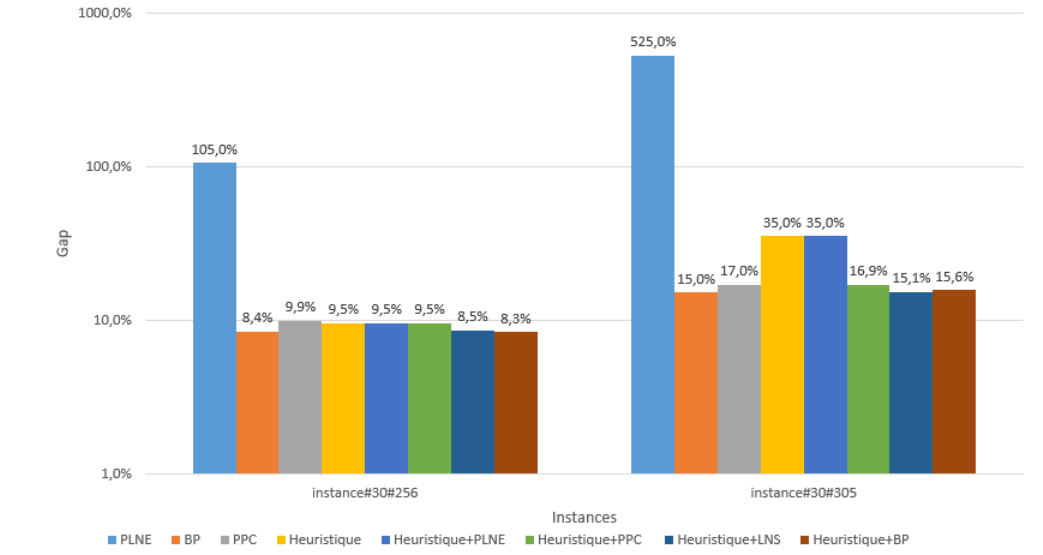
\includegraphics[scale=0.8]{gap.PNG}
\caption{Histogramme représentant le gap obtenu pour chaque instance et modèle utilisé.\label{fig:gap}}
\end{figure}
\end{center}

\newpage
\begin{center}
\begin{figure}
[H]
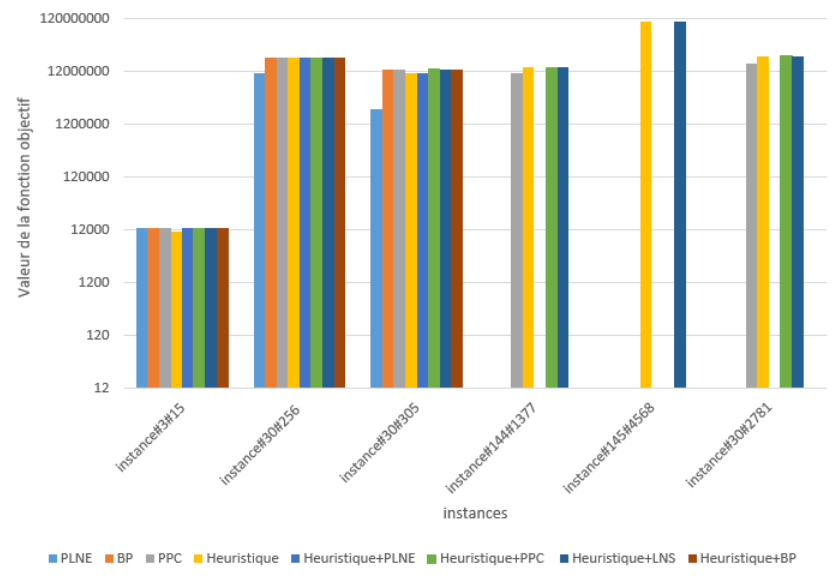
\includegraphics[scale=0.9]{obj.PNG}
\caption{Histogramme représentant la valeur de la fonction objectif obtenue pour chaque instance et modèle utilisé.\label{fig:obj}}
\end{figure}
\end{center}




%%%%%%%%%%%%%%%%%%%%%%%%%%%%%%%%%%%%%%%
%%%%%%%%%%%%%%%%%%%%%%%%%%%%%%%%%%%%%%%




